\documentclass[mathserif,10pt]{beamer}
\hypersetup{pdfmode=FullScreen}
%\usepackage{pgfpages}
%\usepackage{qtree}

\mode<presentation>
{
  \usetheme{shadow}
  \usecolortheme{crane}
  \setbeamercovered{transparent}
  \useoutertheme{infolines}
}

\usepackage{times}
\usepackage{graphicx}
\usepackage[T1]{fontenc}
\usepackage{amssymb,amsmath,amsthm, amsbsy, bm,dsfont}
\newcommand{\bs}{\boldsymbol}
\newcommand{\dd}{\mathrm{d}}
\beamertemplatenavigationsymbolsempty
\DeclareMathOperator{\maximize}{maximize}
\DeclareMathOperator{\E}{\mathbb{E}}
\DeclareMathOperator{\V}{V\mathbb{V}}
\DeclareMathOperator{\VaR}{VaR}
\DeclareMathOperator{\CVaR}{CVaR}




%for R Syntaxhighlighting
\usepackage{listings}
\usepackage{color}


\lstdefinelanguage{R}%
  {keywords={c,list, matrix, nrow,ncol,rownames,colnames,nelson_estim, print, summary, plot},%
   otherkeywords={!,!=,~,$,*,\&,\%/\%,\%*\%,\%\%,<-,<<-,_,/},%
   alsoother={._$},%
   sensitive,%
   morecomment=[l]\#,%
   morestring=[d]",%
   morestring=[d]'% 
  }







\title[Term Structure and Credit Spread Estimation with R]{Term Structure and Credit Spread \\Estimation with R}

\author[Robert Ferstl\and Josef Hayden]{Robert Ferstl\inst{1} \and Josef Hayden\inst{2}}


\institute[]{
\inst{1}Institute for Operations Research\\
Vienna University of Economics and Business Administration
\and
\inst{2}Financial Engineering and Derivatives Group\\
Vienna University of Economics and Business Administration}

\date[AWG]{\scriptsize\em \textbf{First R/Rmetrics User and Developer Workshop\\Meielisalp, Lake Thune, Switzerland\\\vspace{0.2cm} July 8-12, 2007}}

\pgfdeclareimage[height=1.0cm]{wu-logo}{wu-logo}
%\logo{\pgfuseimage{wu-logo}}	% show logo

%\setbeameroption{show notes}
\setbeameroption{hide notes}


\begin{document}
%define colors for syntax highlighting
\definecolor{darkblue}{rgb}{0,0,.5}
\definecolor{darkred}{rgb}{0.4,0.0,0}
\definecolor{commentcolor}{rgb}{0,0.5,0.25}
\definecolor{stringcolor}{rgb}{0.5,0.0,0}

\definecolor{myblue}{rgb}{.8, .8, 1}
\newcommand*\mybluebox[1]{%
\colorbox{myblue}{\hspace{1em}#1\hspace{1em}}}


%settings for R syntaxhighlighting
\lstset{basicstyle=\ttfamily\small,
keywordstyle=\bfseries\color{darkblue},
stringstyle=\ttfamily,
showstringspaces=false,
language=R,
identifierstyle=,
commentstyle=\color{commentcolor},
stringstyle=\color{stringcolor}}





\frame{\titlepage}

\section<presentation>*{Outline}

\begin{frame}
  \frametitle{Outline}
  \tableofcontents[pausesections]
\end{frame}

\section{Introduction}

\subsection{Basic Principles of Bond Pricing}

\begin{frame}
  \frametitle{Basic Principles of Bond Pricing}
  \begin{itemize}
    \item coupon bond which matures in $n$ years
    \item investor gets cashflows $c_t$ at the times $t=1,\dots n$ ($c_n$ includes the redemption payment)
      \item \textcolor{craneblue}{\textbf{clean price}} $p_c$ is quoted on the market
    \item seller also receives \textcolor{craneblue}{\textbf{accrued interest}} for holding the bond over the period since the last coupon payment
  	\begin{equation*}
  \label{accruedinterest}
  a=\frac{\mbox{number of days since last coupon}}{\mbox{number of days in current coupon period}}C
\end{equation*}
	\item investor has to pay the \textcolor{craneblue}{\textbf{dirty price}} $p_d$
\item bond pricing equation with continuous compounding
\begin{equation*}
  \label{bondpriceeq}
  p_c+a = \sum_{t=1}^n \ c_t e^{-s_tm_t}
\end{equation*}
\end{itemize}
\end{frame}

\begin{frame}
\frametitle{Basic Principles of Bond Pricing}
  \begin{itemize}
\item \textcolor{craneblue}{\textbf{yield to maturity}}
\begin{equation*}
  \label{yield}
   p_c+a=\sum_{t=1}^n \ c_t e^{-ym_t}
\end{equation*}
\item  equivalent formulation of the bond price equation uses the \textcolor{craneblue}{\textbf{discount factors}} $d_t=\delta(m_t)=e^{-s_tm_t}$
\item continuous \textcolor{craneblue}{\textbf{discount function}} $\delta(\cdot)$ is formed by interpolation of the discount factors
  \begin{equation*}
  \label{bondprceq2}
    p_c+a=\sum_{t=1}^n \ c_t \delta(m_t) 
  \end{equation*}
   \item \textcolor{craneblue}{\textbf{duration}} is a weighted average of time to cash flows
  \begin{equation*}
 \label{duration} D=\frac{1}{p_c+a}\left[C\sum_{i=1}^n\delta(m_i)m_i+\delta(m_n)Rm_n\right]
\end{equation*}
\end{itemize}
\end{frame}

\subsection{Term Structure Estimation}

% show data set
% data(eurobonds)
% str(eurobonds)

\begin{frame}
	\frametitle{Term Structure Estimation Procedure \newline Notation I}
	\begin{beamerboxesrounded}[shadow=true]{Maturity matrix $\bm{M}$}
		\begin{equation*}\label{maturitym}
		\bm{M}_{\left[n\times m\right]} = \{m_{ij}\}
		\end{equation*}
	\end{beamerboxesrounded}
	
	\vspace{0.3cm}
	\begin{beamerboxesrounded}[shadow=true]{Cashflow matrix $\bm{C}$}
		 \begin{equation*}\label{cashflowm}	
		\bm{C}_{\left[n\times m\right]} = \{c_{ij}\}
		\end{equation*}
	\end{beamerboxesrounded}
	
	\vspace{0.3cm}
	\begin{beamerboxesrounded}[shadow=true]{Clean price vector $\bm{p}^c$}
		 \begin{equation*}\label{pc}
		\bm{p}^c_{\left[1\times m\right]} = \{p^c_j\}
		\end{equation*}
	\end{beamerboxesrounded}	
	
	\vspace{0.3cm}
	\begin{beamerboxesrounded}[shadow=true]{Accrued interest vector $\bm{a}$}
		\begin{equation*}\label{a}
		\bm{a}_{\left[1\times m\right]} = \{a_j\}
		\end{equation*}
	\end{beamerboxesrounded}
	
\end{frame}


\begin{frame}
	\frametitle{Term Structure Estimation Procedure \newline Notation II}
	
	\vspace{0.2cm}
	\begin{beamerboxesrounded}[shadow=true]{Dirty price vector $\bm{p}^d$}
		\begin{equation*}\label{pd}
   		\bm{p}^d_{\left[1\times m\right]}= \{p^d_j\}
		\end{equation*}
		\begin{displaymath}
		\bm{p}^d=\bm{p}^c+\bm{a}
		\end{displaymath}
	\end{beamerboxesrounded}
	
	\vspace{0.2cm}
	\begin{beamerboxesrounded}[shadow=true]{Discount factor matrix $\bm{D}$}
		\begin{equation*}\label{discountm}
		\bm{D}_{\left[n\times m\right]} = \{d_{ij}\}; \qquad d_{ij}=e^{-m_{ij}s(m_{ij},\bm{b})}
		\end{equation*}
	\end{beamerboxesrounded}	
	
	\end{frame}

\section{Nelson/Siegel and Svensson Method}
\subsection{Notation}
\begin{frame}
	\frametitle{Spotrate Functions}
	\begin{block}{Nelson/Siegel:}
	\begin{equation*}\label{nelson}
   	 s(m,\bm{b}) = \beta_0 + \beta_1\frac{1-\exp(-\frac{m}{\tau_1})}{\frac{m}{\tau_1}} + \beta_2\left(\frac{1-\exp(-\frac{m}{\tau_1})}{\frac{m}{\tau_1}} - 	\exp(-\frac{m}{\tau_1})\right)
	\end{equation*}
	\end{block}
	
	\begin{block}{Svensson:}
	\begin{multline*}\label{svspot}
  	  s(m,\bm{b}) = \beta_0 + \beta_1\frac{1-\exp(-\frac{m}{\tau_1})}{\frac{m}{\tau_1}} + \beta_2\left(\frac{1-\exp(-\frac{m}{\tau_1})}{\frac{m}{\tau_1}} - 	\exp(-\frac{m}{\tau_1})\right) \\+ \beta_3\left(\frac{1-\exp(-\frac{m}{\tau_2})}{\frac{m}{\tau_2}} - \exp(-\frac{m}{\tau_2})\right)
	\end{multline*}
	\end{block}
\end{frame}


\begin{frame}
	\frametitle{Minimisation of the weighted pricing errors}
	\vspace{0.2cm}
	\begin{beamerboxesrounded}[shadow=true]{Weights vector $\bm{w}$}
		\begin{equation*}\label{weights}
   		\bm{w}_{\left[1\times m\right]}= \{w_j\}; \qquad   w_j=\frac{\frac{1}{D_j}}{\sum_{i=1}^m\frac{1}{D_i}}
		\end{equation*}
	\end{beamerboxesrounded}	
	
	\begin{block}{Objective function}
	\begin{equation*}
	F= \left(\left(\bm{\iota}_{\left[1 \times n\right]}\left[\bm{C}\cdot\bm{D}\right] - 		\bm{p}^d\right)^2 \bm{w}\bm{\iota}_{\left[m \times 1\right]} \right)
		 \end{equation*}
	\end{block}
    	\begin{block}{Minimisation problem}
	 $$\min_{\mathbf{b} \in G} F(\mathbf{b}) $$
	 $$ \mathbf{b} \in G =   \{ \mathbf{b} \in \mathds{R}^4 ; \mathds{R}^6 : \mathbf{lb} \leq \mathbf{b} \leq \mathbf{ub}  \}$$
	\end{block}
	
	\begin{block}{Parameter constraints}
	$$\beta_0 >0, \tau_1>0, \tau_2>0$$
	\end{block}
	

\end{frame}


\subsection{Example}

\begin{frame} [containsverbatim]\frametitle{Example}
  % \beamergotobutton{boxmuller}

\begin{lstlisting}
data(eurobonds)

group <- c("GERMANY", "AUSTRIA", "ITALY")
bonddata <- eurobonds
matrange <- c(2,10)
method <- "Nelson/Siegel"
fit <- "prices"
weights <- "none"
control <- list(eval.max=100000)

b <- matrix(c(0.02, -0.01, -0.025,  1,
 			0.026, -0.011, -0.0262,    1,
			0.025, -0.015, -0.025,    1),
			nrow=3,ncol=4,byrow=TRUE)
			
rownames(b) <- group

colnames(b) <- c("beta0","beta1","beta2","tau1")
x <- nelson_estim(group, bonddata, matrange, 
                  method, fit, weights, startparam=b,control)
\end{lstlisting}
\end{frame}


\section{Cubic Splines}

\subsection{Notation}



\section{Conclusion}






% \begin{frame}
%   \frametitle{Term structure and credit spread estimation} 
%   \begin{itemize}
%   \item estimate zero-coupon yield curves and credit spread curves from market data
%   \item usual way for calculation of \textcolor{craneblue}{\textbf{credit spread curves}} 
%   \end{itemize}
% \begin{equation*}
%   \label{spread}
% cs_j(\bm{m}) = s_j(\bm{m,b}) - s_{ref}(\bm{m,b})
% \end{equation*}

%  \vspace{0.5cm}
% \begin{tabular}{ll}
% $cs_j(\bm{m})$ & credit-spread between country $j$ and reference country $ref$ \\
% $s_j(\bm{m,b})$ &spot-rate curve of country $j$ with maturity vector  $\bm{m}$ \\
% $s_{ref}(\bm{m,b})$ & spot-rate curve of the reference country
% \end{tabular}


% %\begin{center}
% %	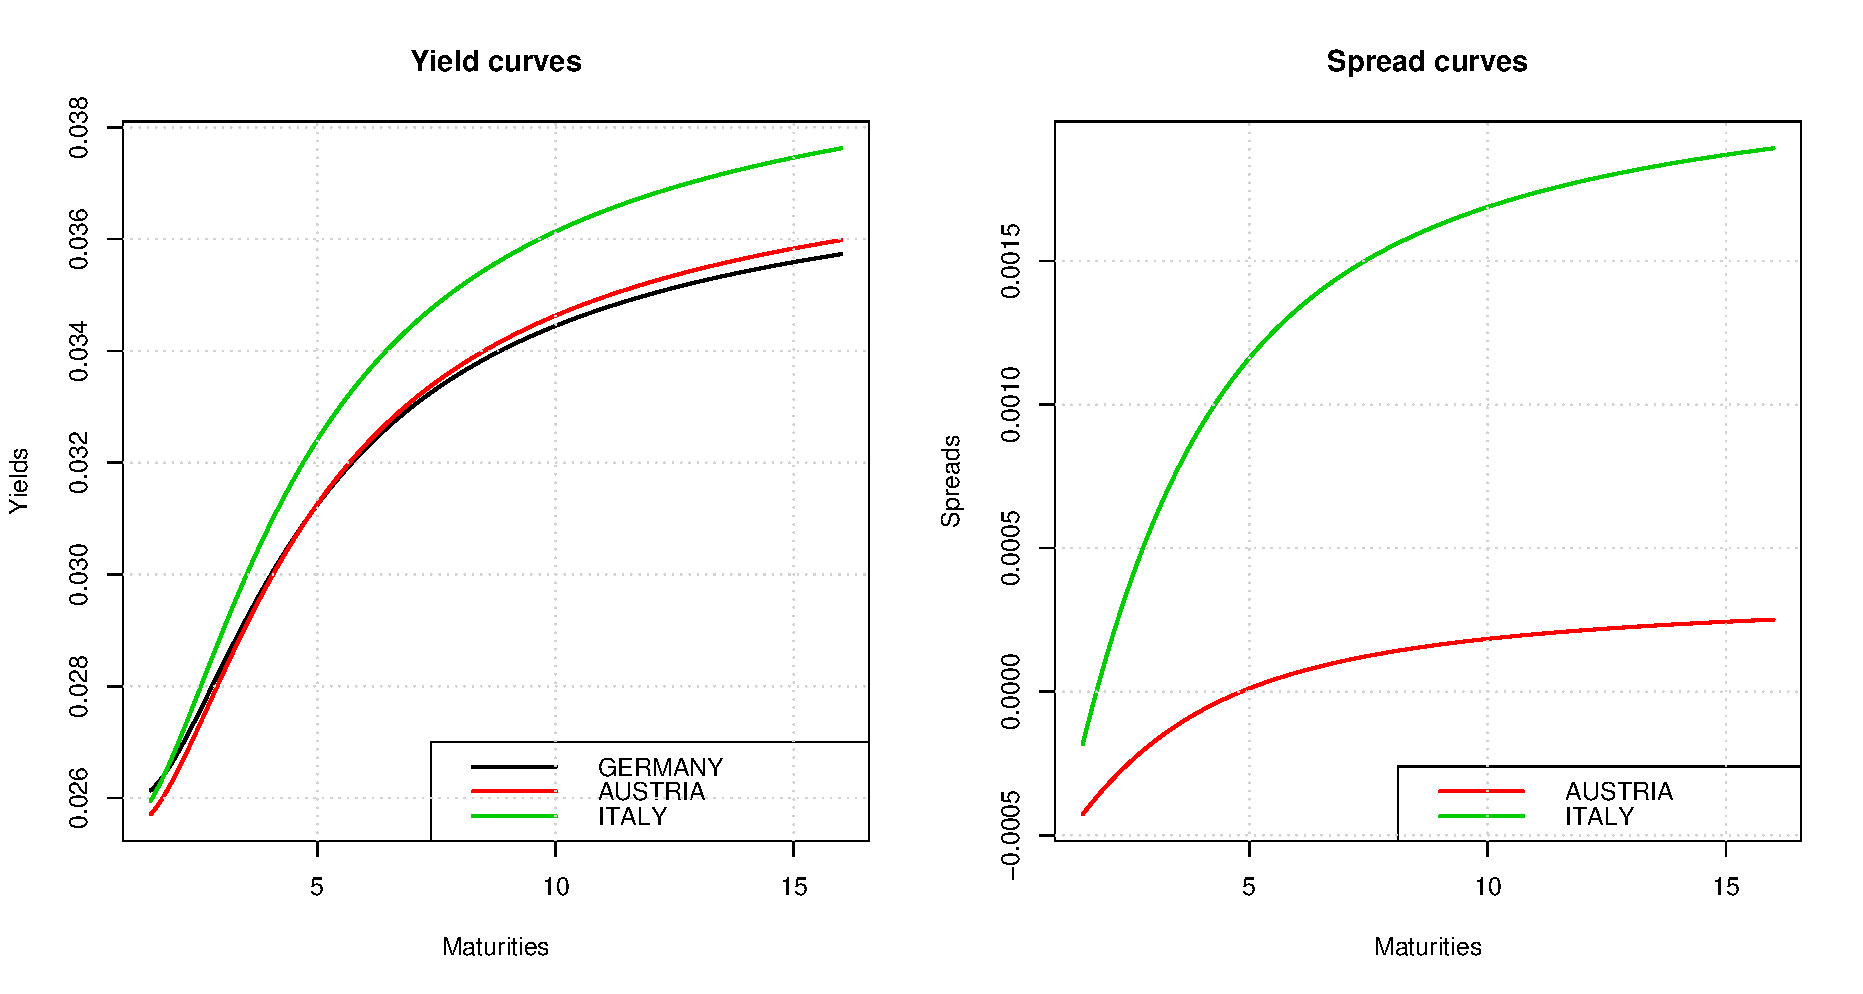
\includegraphics[width=0.97\textwidth]{curves}
% %\end{center}
% \end{frame}


% \begin{frame}
%   \frametitle{Nelson and Siegel (1987) approach}
%   %\framesubtitle{Untertitel sind optional.}
%    \begin{beamerboxesrounded}[shadow=true]{Instantaneous forward rates}
% \begin{equation*}
% 	    f(m,\bm{b}) = \beta_0 + \beta_1 \exp(-\frac{m}{\tau_1}) + \beta_2 \frac{m}{\tau_1} \exp(-\frac{m}{\tau_1})
% \end{equation*}
%  \end{beamerboxesrounded} 

%  \vspace{1.5cm}

% \begin{beamerboxesrounded}[shadow=true]{Spot rates}
% \begin{equation*}\label{nelson}
%     s(m,\bm{b}) = \beta_0 + \beta_1\frac{1-\exp(-\frac{m}{\tau_1})}{\frac{m}{\tau_1}} + \beta_2\left(\frac{1-\exp(-\frac{m}{\tau_1})}{\frac{m}{\tau_1}} - \exp(-\frac{m}{\tau_1})\right)
% \end{equation*}
% \end{beamerboxesrounded}

% %\begin{center}
% %	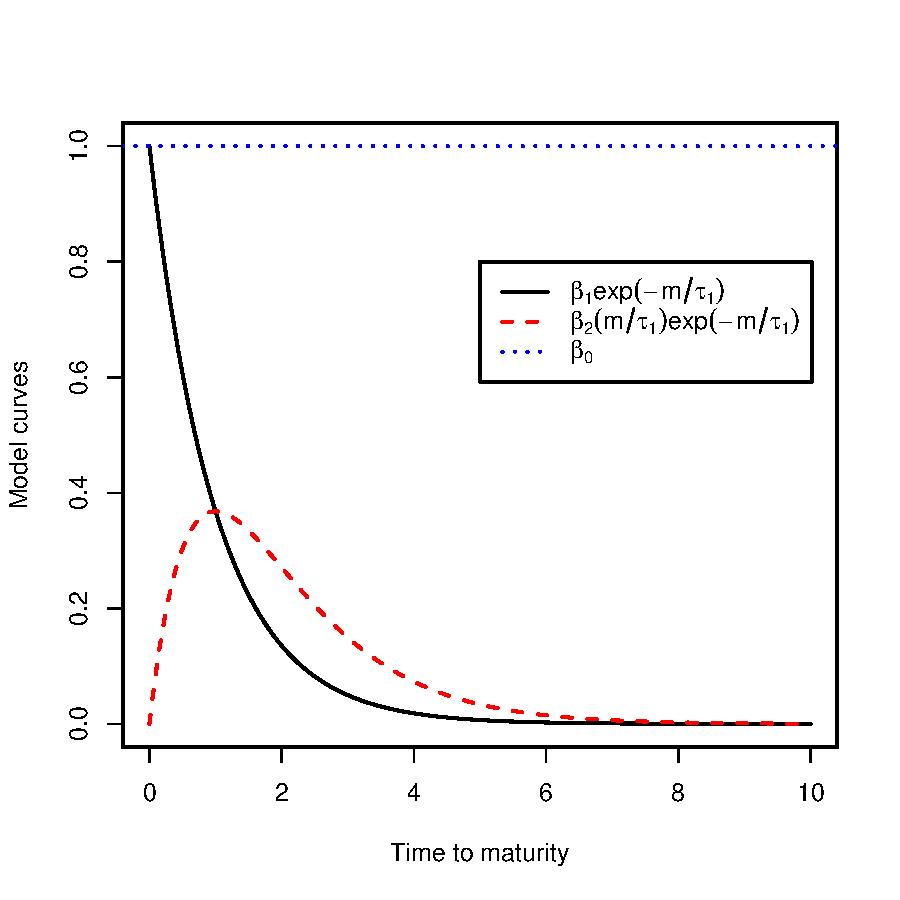
\includegraphics[width=0.65\textwidth]{fignelson}
% %\end{center}
% \end{frame}


% \begin{frame}
%   \frametitle{Svensson (1994) approach}
%  \begin{itemize}
%    \item Svensson (1994) extended the functional form by two additional parameters which allows for a second hump-shape
%  \end{itemize}

% \begin{beamerboxesrounded}[shadow=true]{Instantaneous forward rates}
% \begin{equation*}
% 	    f(m,\bm{b}) = \beta_0 + \beta_1 \exp(-\frac{m}{\tau_1}) + \beta_2 \frac{m}{\tau_1} \exp(-\frac{m}{\tau_1})+\beta_3 \frac{m}{\tau_2} \exp(-\frac{m}{\tau_2})
% \end{equation*}
% \end{beamerboxesrounded}
% \vspace{0.5cm}
% \begin{beamerboxesrounded}[shadow=true]{Spot rates}
% \begin{multline*}\label{svspot}
%     s(m,\bm{b}) = \beta_0 + \beta_1\frac{1-\exp(-\frac{m}{\tau_1})}{\frac{m}{\tau_1}} + \beta_2\left(\frac{1-\exp(-\frac{m}{\tau_1})}{\frac{m}{\tau_1}} - \exp(-\frac{m}{\tau_1})\right) \\+ \beta_3\left(\frac{1-\exp(-\frac{m}{\tau_2})}{\frac{m}{\tau_2}} - \exp(-\frac{m}{\tau_2})\right)
% \end{multline*}
% \end{beamerboxesrounded}
% \end{frame}

% \begin{frame}
% 	\frametitle{Decomposition of the Svensson forward rate function}
	
% 	\begin{center}
% 	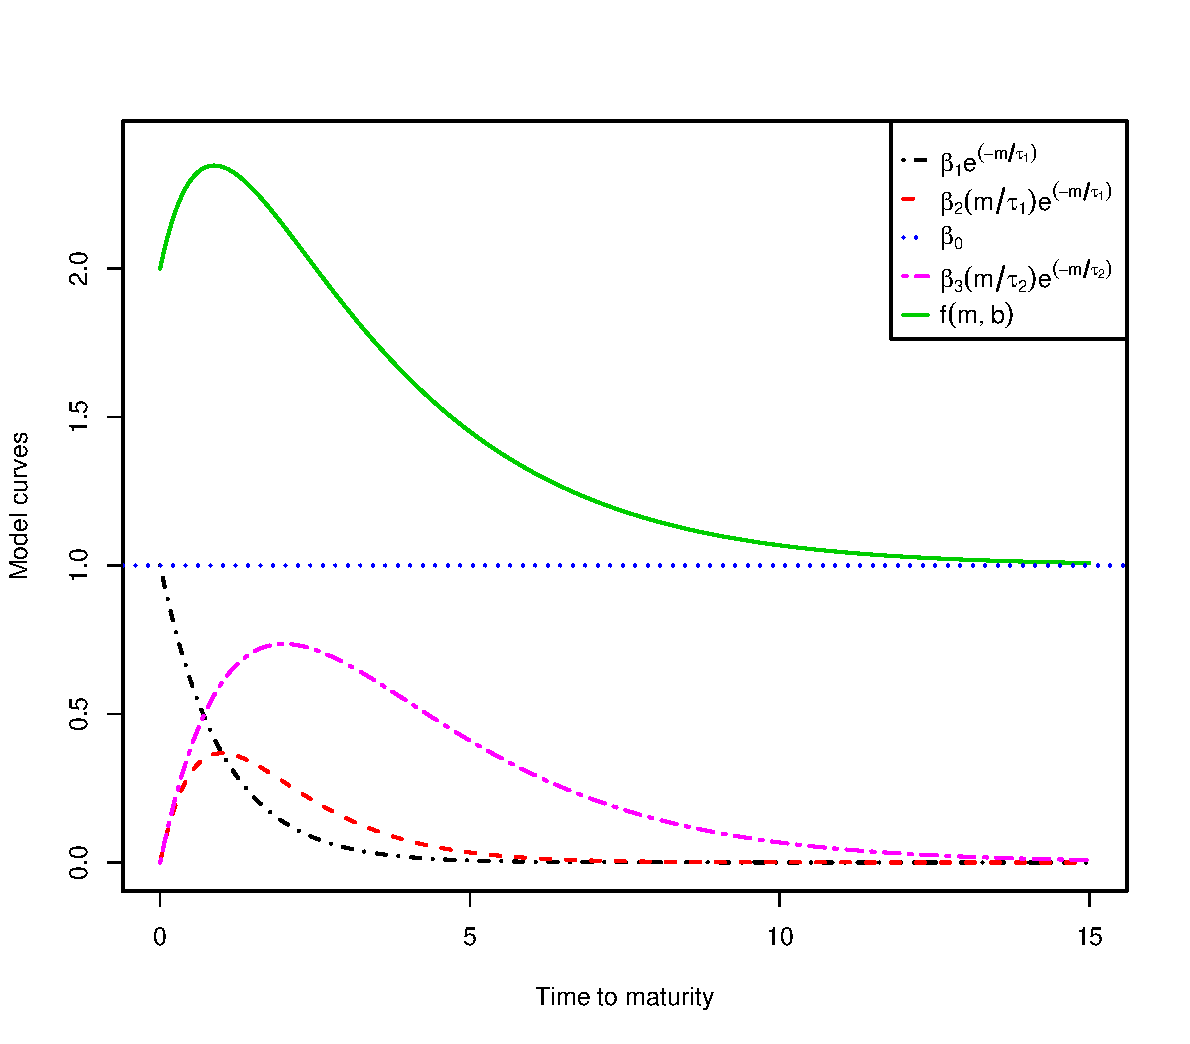
\includegraphics[width=0.8\textwidth]{sv.pdf}
% 	\end{center}

% \end{frame}




% \begin{frame}
% 	\frametitle{Term structure estimation procedure \newline Objective function}

% 	\begin{itemize}
% 		\item Minimization of the weighted pricing or yield errors
% 	\end{itemize}
% 	\begin{beamerboxesrounded}[shadow=true]{Objective function}
% 		\begin{equation*}
% 		 \bm{b}_{opt} = \min_{b}\left(\left(\bm{\iota}_{\left[1 \times n\right]}\left[\bm{C}\cdot\bm{D}\right] - 		\bm{p}^d\right)^2 \bm{w}\bm{\iota}_{\left[m \times 1\right]} \right)
% 		 \end{equation*}
% 	\end{beamerboxesrounded}
	
% 	\begin{itemize}
% 		\item The parameter vector is subject to constraints ($\beta_0 >0, \tau_1>0, \tau_2>0$)
% 	\end{itemize}


% \end{frame}





\begin{frame}
	\frametitle{Examples}
\end{frame}

\begin{frame}[allowframebreaks]
 \frametitle<presentation>{References}

  \begin{thebibliography}{10}

  \scriptsize
  \beamertemplatearticlebibitems
  
  





%Charles R. Nelson and Andrew F. Siegel (1987): Parsimonious modeling of yield curves. The Journal of Business, 60(4):473�489.

%Lars E.O. Svensson (1994): Estimating and interpreting forward interest rates: Sweden 1992 -1994. Technical Reports 4871, National Bureau of Economic Research.
  
  
  
   \bibitem{BIS2005}
   Bank for International Settlements
   \newblock Zero-coupon yield curves: technical documentation
   \newblock {\em BIS Papers}, No. 25, October 2005
   
   \bibitem{Bliss2007}
   Robert R. Bliss 
   \newblock Testing term structure estimation methods. 
   \newblock {\em Advances in Futures and Options Research}, No. 9, p. 197--232 , 2007
  
  \bibitem{Bolder1999}
   David Bolder, David Streliski
   \newblock Yield Curve Modelling at the Bank of Canada
   \newblock {\em Bank of Canada, Technical Report}, No. 84, 1999
  
    \bibitem{Geyer1999}
   Alois Geyer, Richard Mader
    \newblock Estimation of the Term Structure of Interest Rates - A Parametric Approach
    \newblock {\em OeNB, Working Paper}, No. 37, 1999

  \bibitem{Jankowitsch2004}
    Rainer Jankowitsch, Stefan Pichler
    \newblock Parsimonious Estimation of Credit Spreads
    \newblock {\em The Journal of Fixed Income}, 14(3):49--63, 2004
    
    \bibitem{Ioannadis2003}
    Michalis Ioannides
    \newblock A comparison of yield curve estimation techniques using UK data.
    newblock {\em Journal of Banking \& Finance}, 27, 1--26
    
    \bibitem{McCulloch1971}
    J. Huston McCulloch
    \newblock Measuring the Term Structure of Interest Rates
    \newblock {\em The Journal of Business}, 44, 19--31
    
     \bibitem{McCulloch1975}
    J. Huston McCulloch
    \newblock  The Tax-Adjusted Yield Curve
    \newblock {\em The Journal of Finance}, 30, 811--830
    
    \bibitem{Nwalkhaetal2005}
     Sanjay K. Nawalkha and Gloria M. Soto and Natalia K. Beliaeva
     \newblock Interest Rate Risk Modeling
     \newblock{\em The Fixed Income Valuation Course}, Wiley Finance 2005
      
    \bibitem{Nelson1987}
    Charles R. Nelson, Andrew F. Siegel
    \newblock Parsimonious Modeling of Yield Curves
    \newblock {\em The Journal of Business}, 60(4):473--489, 1987
    
    \bibitem{Svensson1994}
    Lars E.O. Svensson
    \newblock Estimating and Interpreting Forward Interest Rates:\\Sweden 1992 -1994
    \newblock {\em National Bureau of Economic Research, \\Technical Report}, No. 4871, 1994

  \end{thebibliography}
\end{frame}

\end{document}
